\documentclass[a4paper, 11pt]{article}

\title{\scshape{} Informe Ejercio Electroneum\'atica y Rel\'e Logo}
\date{\scshape{} 05/11/2021}
\author{\scshape{} Sebastian Castellanos y Stiven Perez}

% Declaracion de paquetes a usar
\usepackage[utf8]{inputenc}
\usepackage[spanish]{babel}
\usepackage[margin=2cm, top=2cm,includefoot]{geometry}
\usepackage[hidelinks]{hyperref}
\usepackage{graphicx} % insercion de imagenes
\usepackage[table, xcdraw]{xcolor} % deteccion de colores
\usepackage{fancyhdr} % estilo de pagina
\usepackage{parskip} % arreglado de tabs en el text
\usepackage[figurename=Figure]{caption} % editar nombre del caption
\usepackage{pdfpages}
\usepackage{setspace}
% Declaracion de variables
\newcommand{\startDate}{08/10/2021}
\newcommand{\logoLeft}{images/logo-logo.jpg}
\newcommand{\logoRight}{images/sena.png}
\newcommand{\ejercicio}{images/ejercicio.png}
\newcommand{\ecuacion}{images/ecuacionNeumatica.jpg}
\newcommand{\simulacion}{simulacion.pdf}
\newcommand{\program}{bloques.pdf}
\newcommand{\esquema}{esquema.pdf}
\newcommand{\inputs}{images/io.png}
% Declaracion de colores
\definecolor{greenPortada}{HTML}{69A84F}

% adicionales
\setlength{\headheight}{46.2pt} % espaciado del encabezado de forma vertical
\pagestyle{fancy}
\fancyhf{}
\lhead{\includegraphics[width=1.9cm]{\logoLeft}} % imagen en el encabezado, lado izquierdo
\rhead{\includegraphics[width=1.5cm]{\logoRight}} % imagen en el encabezado, lado derecho
\renewcommand{\headrulewidth}{3pt} % ancho de la linea horizontal del encabezado
\renewcommand{\headrule}{\hbox to\headwidth{\color{greenPortada}\leaders\hrule height \headrulewidth\hfill}} % color de la linea horizontal del encabezado

% // -> define un salto de linea en el parrafo
% vfill -> aprovechar espacios en blanco

% start document
\begin{document}
  \maketitle{\scshape{}}
  \cfoot{\thepage}
% indice ------------------------------------------------------
\clearpage{}
\tableofcontents{}
\clearpage{}
% ------------------------------------------------------- 
\section{Planteamiento}
Se tiene una maquina fresadora y taladradora, se requiere automatizar con el fin de que el operario solo ingrese la pieza a trabajar en el apartado de la mesa, pulsar el boton de start e inicie todo el proceso de taladro y fresa. Se dispone de 3 (A,B Y C) cilindros neumáticos de doble efecto y se ubicarán como indica la imagen.
\vfill{}
\begin{figure}[h]
  \centering{}
  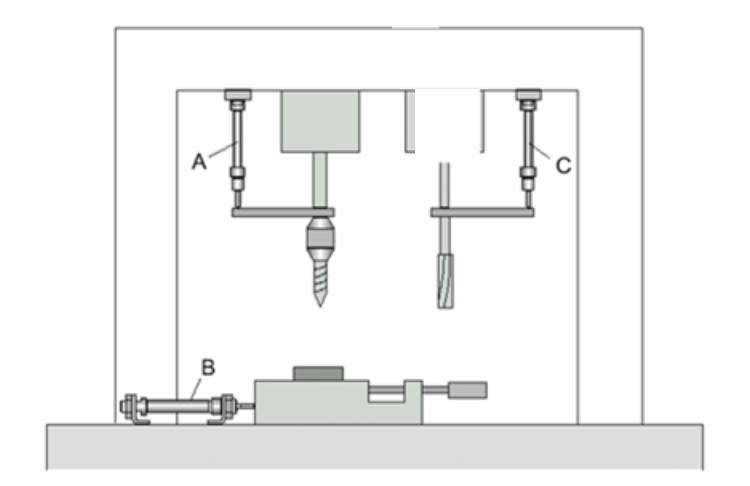
\includegraphics[width=\textwidth]{\ejercicio}
  \caption{exposición inicial.}
\end{figure}
\vfill{}
\section{Desarrollo}
Para poder realizar una adecuada automatización con los cilindros neumáticos, se analizó el proceso y se hallo la siguiente ecuación neumática desarrollada por el metodo cascada.
\vfill{}

\clearpage{}
\subsection{Ecuación Neumática}
\vfill{}
\begin{figure}[h]
  \centering{}
  \includegraphics[width=0.5\textwidth]{\ecuacion}
  \caption{Ecuación Neumática.}
\end{figure}
\vfill{}
\subsection{Entradas y salidas Logo}
En la siguiente tabla se encuentra en que entrada (I) y que salida (Q) estara cada pulsador y contacto de los sensores reed asi como las respectivas bobinas solenoides de las electrovalvulas.
\begin{figure}[h]
  \centering{}
  \includegraphics[width=0.98\textwidth{}]{\inputs}
  \caption{Inputs - Outputs.}
\end{figure}
\clearpage{}
\subsection{Diseño y simulación en FluidSim}
Hallando la ecuación neumática procedemos a realizar el diseño y posteriormente la simulación en el software FluidSim, se hará uso de tres cilindros neumáticos de doble efecto, 3 valvulas biestables, el rele programable Logo, un pulsador NO para la señal de START, un pulsador NC para la señal de STOP, bobinas solenoides de las respectivas electrovalvulas y sensores reed con sus recpectivos contactos cableados al Logo.

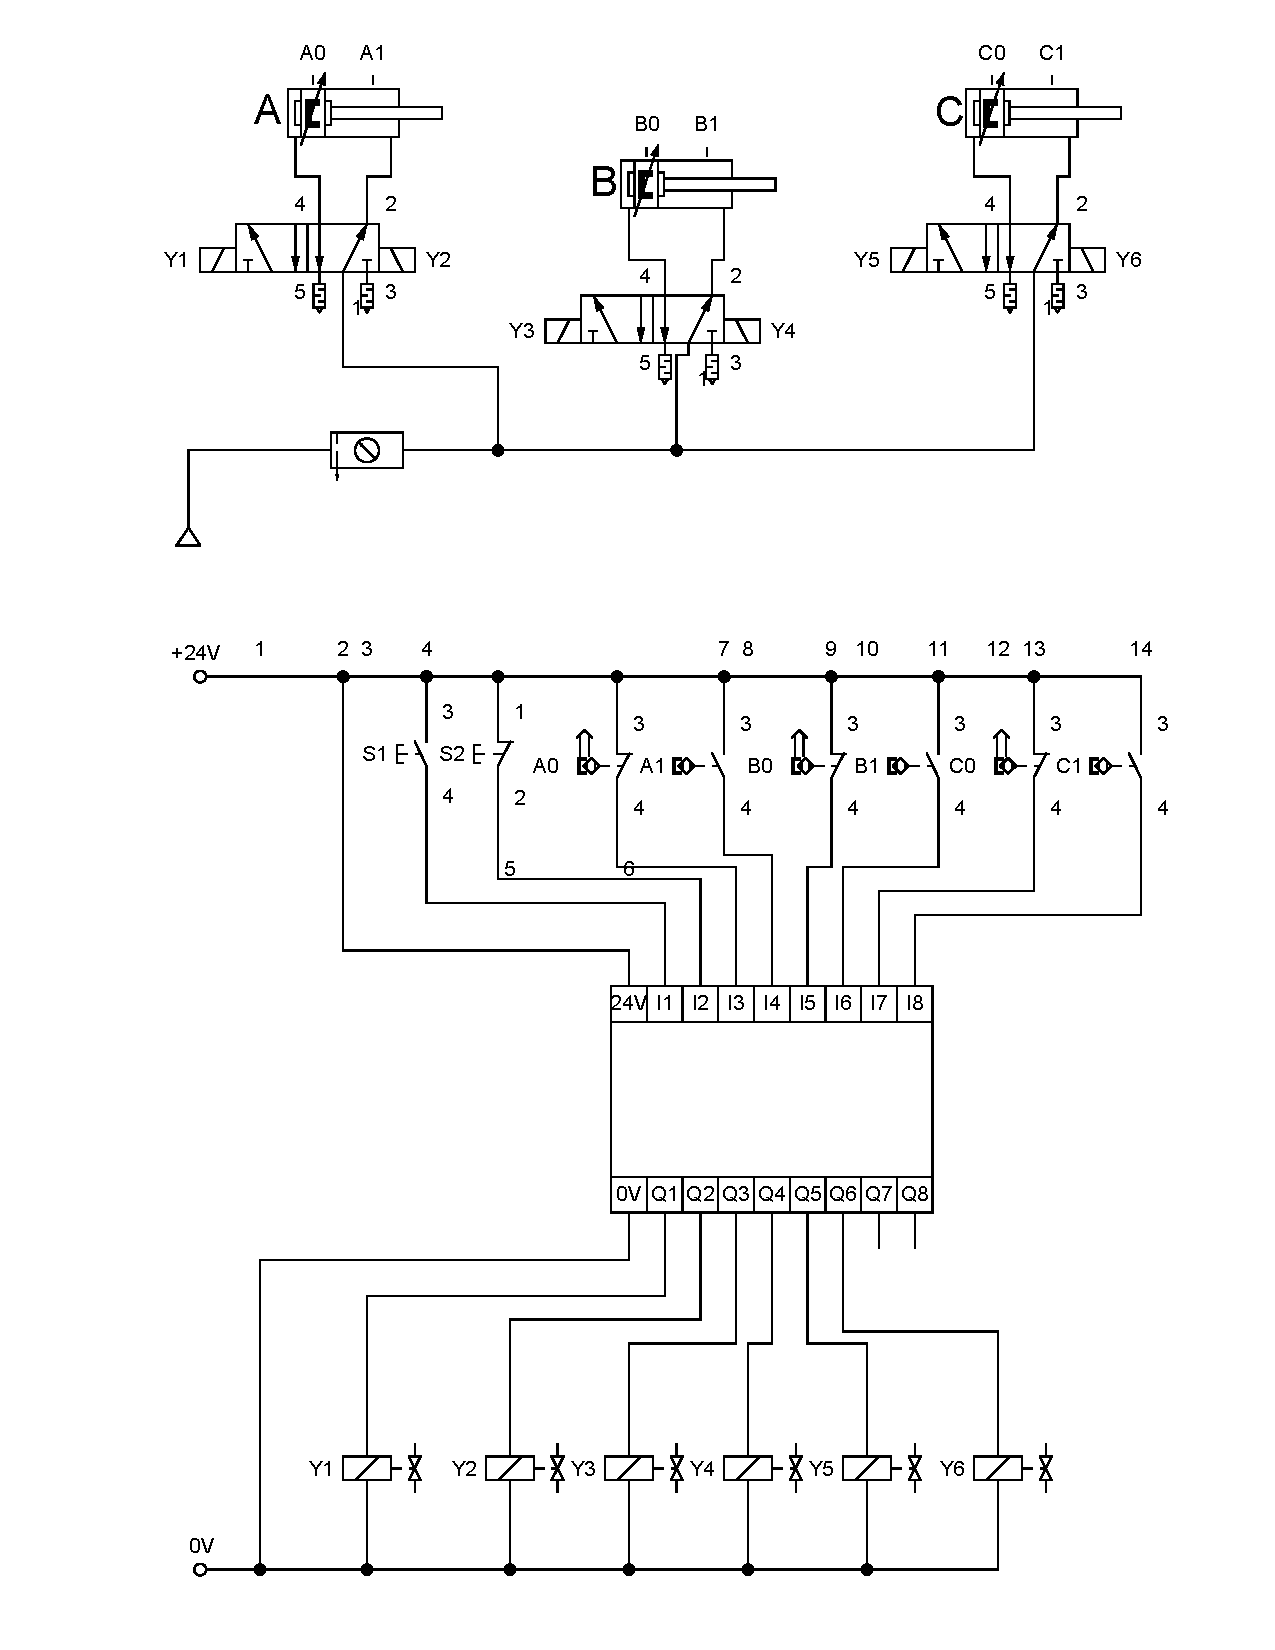
\includepdf[pages=-]{\simulacion}

\subsection{Programación Logo}
La programación de la secuencia se realizo por el lenguaje de diagrama de bloques funcionales (FBD).
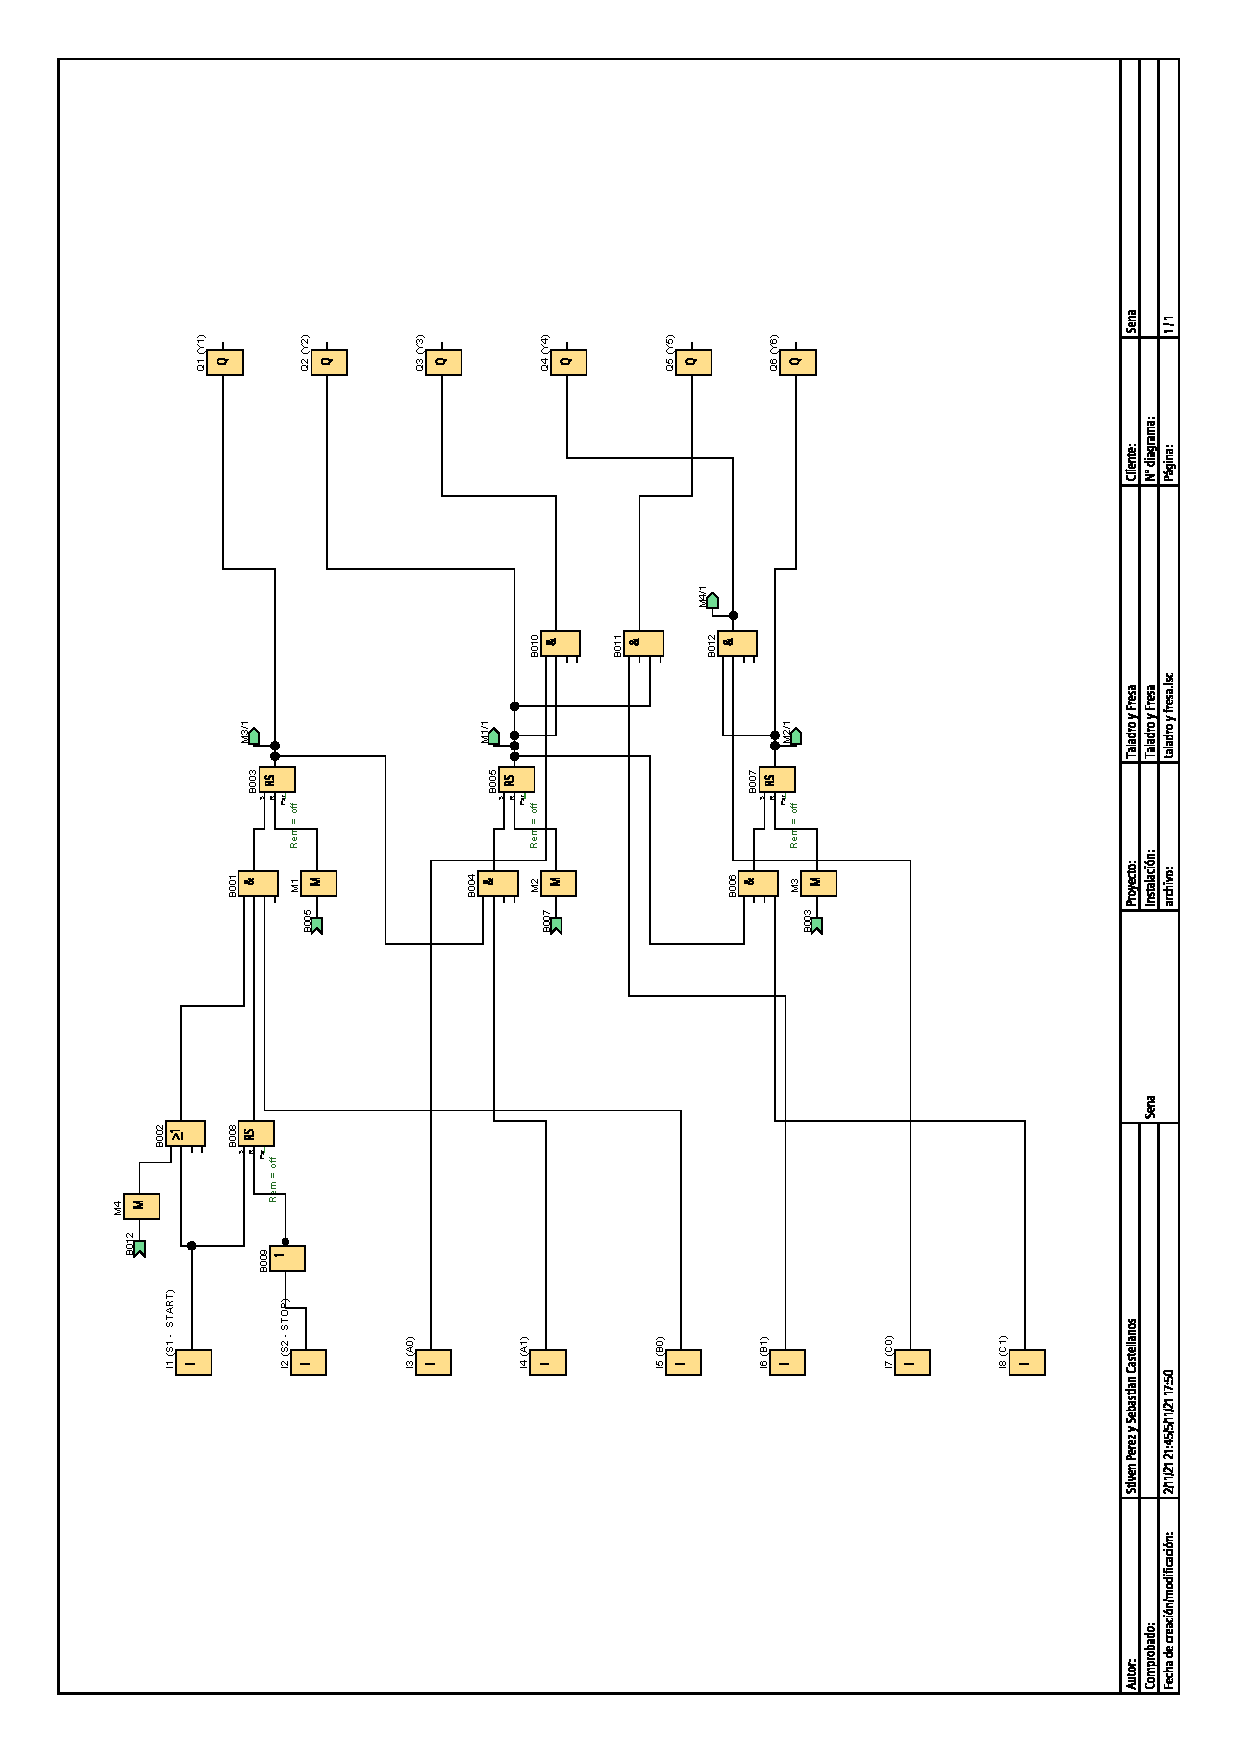
\includepdf[pages=-]{\esquema}

\end{document}
